%-----------------------------------------------------------------------------%
\chapter{\babEmpat}
\label{bab:4}
%-----------------------------------------------------------------------------%
Bab ini membahas desain dan implementasi sistem dalam penelitian ini. Pembahasan
dilakukan mulai dari proses pembuatan \textit{delivery order}, rancangan arsitektur sistem, dan rancangan simulasi. Dilanjutkan dengan pembahasan simulasi blockchain, dan desain evaluasi dari sistem INSW yang dikembangkan. Untuk ringkasan simulasi dapat dilihat di akhir bab ini pada Tabel \ref{tab:simulation}.

\section{Proses Pembuatan \textit{Delibery Order}}
\label{sec:proses_do}
Proses pembuatan dimulai dari pengguna akhir membuat permohonan melalui perusahaan maupun aplikasi perusahaan eksportir dan importir. Perusahaan tersebut kemudian mengajukan permohonan ekspor/impor barang ke sistem INSW melalui \textit{peer} milik perusahaan tersebut. Permohonan akan dilakukan pengecekan terhadap aturan-aturan yang ada terhadap barang-barang yang akan diekspor atau diimpor oleh \textit{logic} pada \textit{smart contract}.

\begin{figure}
	\centering
	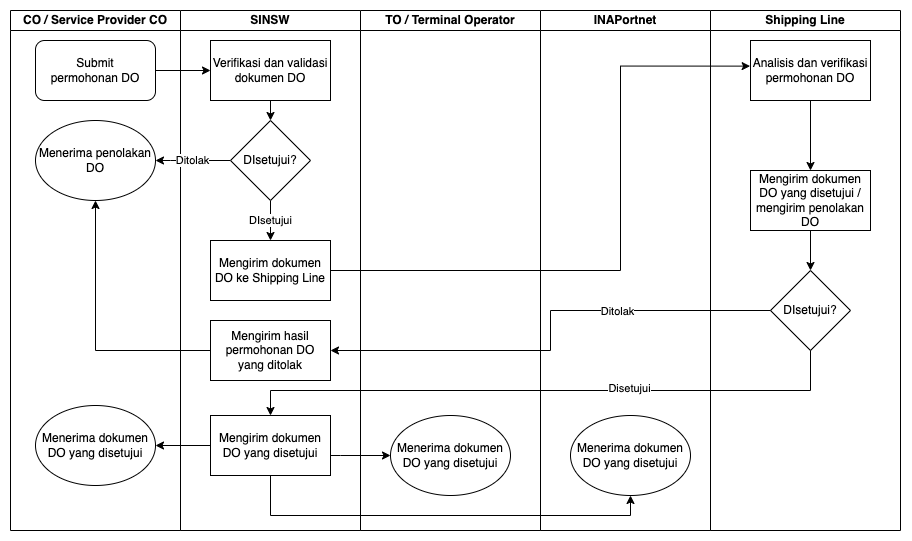
\includegraphics[width=\textwidth]{assets/pics/request_do.drawio.png}
	\caption{Proses pembuatan \textit{delivery order} yang ada.}
	\label{fig:request_do_classic}
\end{figure}

Sebagai perbandingan, \pic~\ref{fig:request_do_classic} merupakan proses permohonan \textit{delivery order} pada sistem INSW saat ini. Gambar tersebut merupakan asumsi penulis yang didasarkan pada situs INSW\footnote{https://insw.go.id/aplikasi-lnsw} untuk digunakan dalam penelitian ini dikarenakan keterbatasan akses terhadap sistem sungguhan. Dapat dilihat pada proses tersebut bahwa setelah dokumen permohonan \textit{delivery order} diunggah, dokumen tersebut masih perlu diverifikasi manual oleh pihak INSW dan \textit{shipping line}. Sedangkan proses pembuatan \textit{delivery order} pada sistem berbasis \textit{blockchain} dapat dilihat pada \pic~\ref{fig:request_do_blockchain_flow}. Pada proses ini proses verifikasi manual dihilangkan dan digantikan oleh \textit{smart contract}.

\begin{figure}
	\centering
	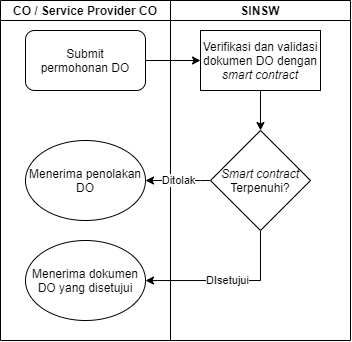
\includegraphics[width=\textwidth]{assets/pics/request_do_blockchain_flow.png}
	\caption{Proses pembuatan \textit{delivery order} yang diajukan.}
	\label{fig:request_do_blockchain_flow}
\end{figure}


\section{Rancangan Sistem \textit{Delivery Order} berbasis \textit{Blockchain}}
\label{sec:rancangansistem}

Pada subbab ini dijelaskan rancangan sistem \textit{delivery order} yang diajukan. Kemudian dijelaskan konfigurasi komponen-komponen Hyperledger Fabric serta infrastruktur yang digunakan untuk pengujian sistem. Rancangan arsitektur dapat dilihat pada \pic~\ref{fig:fabric_arch_imp}. Pemilihan nama digunakan hanya untuk kepentingan simulasi dalam penelitian ini dan tidak merujuk pada dunia nyata.


\begin{figure}
	\centering
	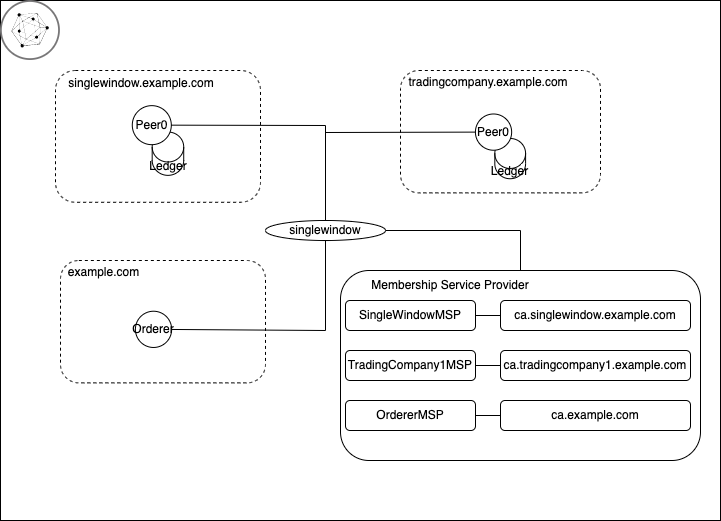
\includegraphics[width=\textwidth]{assets/pics/fabric_arch_imp2}
	\caption{Arsitektur sistem \textit{delivery order} yang dirancangan.}
	\label{fig:fabric_arch_imp}
\end{figure}

%\subsection{\textit{Channel}}
%\label{subsec:channel}

Sistem \textit{delivery order} dirancang menggunakan satu \textit{channel} dengan nama "singlewindow". Konfigurasi \textit{channel} didefinisikan pada \textit{file} bernama configtx.yaml\footnote{https://github.com/fadhilrasendriya/fabric-window/blob/main/test-network/configtx/configtx.yaml}. Konfigurasi \textit{channel} mencakup \textit{organization}, \textit{capabilities}, \textit{orderer}, \textit{application}, dan \textit{profile}.

Untuk konfigurasi organisasi digunakan tiga organisasi yaitu example.com, singlewindow.example.com, dan tradingcompany1.example.com. Setiap organisasi berkontribusi ke jaringan Fabric dengan menyumbang \textit{peer} maupun \textit{orderer}. Organisasi example.com merupakan organisasi dalam jaringan Fabric yang bertugas menjadi \textit{orderer} untuk melaksanakan konsensus. Organisasi selanjutnya adalah singlewindow.example.com yang merepresentasikan perusahaan INSW yang bertugas sebagai administrator \textit{channel}. Sedangkan organisasi tradingcompany1.example.com merepresentasikan perusahaan eksportir dan importir yang bergabung dalam jaringan \textit{blockchain}. Organisasi singlewindow.example.com memiliki wewenang untuk mengatur, membuat, dan mengubah aturan terhadap barang ekspor dan impor.  Sedangkan untuk pengajuan \textit{delivery order}, dilakukan melalui organisasi tradingcompany1.example.com (perusahaan eksportir dan importir). Definisi organisasi dapat dilihat pada configtx.yaml bagian \textit{organization}.


Bagian selanjutnya yaitu konfigurasi \textit{endorsement policy}. Setiap organisasi yang tergabung menyetujui \textit{endorsement policy} ketika melakukan \textit{approve} pada \textit{chaincode} (\textit{smart contract}) yang akan digunakan. Dalam penelitian ini digunakan \textit{endorsement policy} berupa mayoritas dan didefinisikan dalam \textit{channel} agar \textit{endorsement policy} secara otomatis diperbarui ketika organisasi bergabung maupun meninggalkan \textit{channel} \citep{Androulaki2018}.


Komponen selanjutnya yang dibahas adalah \textit{peer}. \textit{Peer} merupakan komponen penting tempat \textit{ledger} disimpan dan sebagai tempat eksekusi \textit{smart contract}. Dalam Hyperledger Fabric terdapat dua jenis \textit{peer}: \textit{orderer} dan normal. \textit{Orderer} adalah jenis \textit{peer} yang bertugas melakukan pengurutan terhadap semua \textit{event} yang terjadi pada \textit{channel}. \textit{Orderer} dalam Fabric menggunakan algoritma konsensus Raft. Sebelumnya, terdapat tiga pilihan algoritma konsensus pada \textit{orderer} yaitu Solo, untuk \textit{orderer singular}, Kafka, dan Raft. Namun, konsensus Solo dan Kafka ditandai sebagai \textit{deprecated} untuk Fabric versi 2.0 ke atas sehingga digunakan konsensus Raft dalam penelitian ini. Selain itu, tipe konsensus Raft sudah tersedia secara \textit{native} dalam \textit{source code orderer} sehingga tidak membutuhkan \textit{setup} ekstra seperti halnya konsensus Kafka serta penggunaan Raft memungkinkannya untuk setiap organisasi berkontribusi menjadi \textit{orderer} \citep{Androulaki2018}. Setiap organisasi dibuatkan satu \textit{peer} dengan rincian sebagai berikut: 1 \textit{orderer} orderer.example.com untuk organisasi example.com, 1 \textit{peer} peer0.singlewindow.example.com untuk organisasi singlewindow.example.com, dan 1 \textit{peer} peer0.tradingcompany1.example.com untuk organisasi tradingcompany1.example.com. Dalam rancangan ini hanya digunakan satu organisasi \textit{orderer}.


Untuk logika aplikasi \textit{blockchain} diimplementasikan menjadi satu \textit{chaincode} bernama do\_chaincode dengan dua \textit{smart contract}: GoodContract dan OrderContract. \textit{GoodContract} mengatur daftar barang dan batas-batas yang diperbolehkan untuk diimpor atau diekspor. Sedangkan OrderContract berisi fungsi untuk membaca dan membuat \textit{delivery order}. \textit{Chaincode} dibuat menggunakan \textit{library} fabric-contract-api-go\footnote{https://github.com/hyperledger/fabric-contract-api-go}. Fungsi-fungsi pada do\_chaincode yang dibuat dapat dilihat pada Tabel \ref{table:smartcontract}. 

\begin{center}
\begin{table}
\caption{Tabel Fungsi \textit{Smart Contract}}
\begin{tabular}{ |c|c|p{5cm}|p{3cm}| } 
 \hline
 \textit{\textbf{Smart Contract}} & \textbf{Fungsi} & \textbf{Deskripsi} & \textbf{Pengakses} \\ 
 \hline
 GoodContract & CreateGood & Melakukan pembuatan \textit{good} (barang) & organisasi INSW \\ 
 \hline
 GoodContract & GetGoodById & Membaca \textit{good} yang ada & anggota \textit{channel} \\ 
 \hline
 OrderContract & CreateOrder & Membuat \textit{delivery order} & INSW dan perusahaan \\
 \hline
 OrderContract & ReadOrder & Membaca \textit{delivery order} & anggota \textit{channel} \\
 \hline
\end{tabular}

\label{table:smartcontract}
\end{table}
\end{center}

%\subsection{Fabric CA Server dan Cryptogen}
%\label{subsec:fabric-ca}

\textit{Sequence diagram} proses pembuatan \textit{delivery order} dapat dilihat pada \pic~\ref{fig:request_do_seq}. Pada proses ini, pengguna akhir (eksportir atau importir) melakukan \textit{submit} permohonan melalui aplikasi suatu perusahaan, yang kemudian perusahaan tersebut meneruskan permohonan dengan memanggil \textit{smart contract} melalui \textit{peer} milik perusahaan tersebut. Kemudian dilakukan proses transaksi sesuai dengan arsitektur Hyperledger Fabric (lihat Subbab \ref{sec:hypefabric}).

\begin{figure}
	\centering
	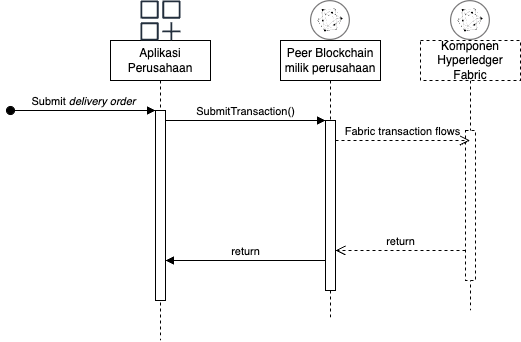
\includegraphics[width=\textwidth]{assets/pics/do_blockchain.drawio.png}
	\caption{\textit{Sequence diagram} proses \textit{delivery order} yang diajukan.}
	\label{fig:request_do_seq}
\end{figure}

Proses autentikasi pada Fabric mengandalkan sertifikat digital untuk menjaga integritas pesan dalam komunikasi antarkomponen Fabric serta transparansi identitas untuk anggota jaringan Fabric. Dalam Fabric terdapat komponen opsional bernama fabric-ca untuk mengatur dan membantu membuat \textit{credential} dan identitas untuk komponen-komponen Fabric. Terdapat juga \textit{tool} bernama cryptogen untuk keperluan \textit{testing} yang digunakan dalam penelitian ini untuk menyediakan CA dan \textit{credential}. Cryptogen dipilih sebagai penyedia CA dikarenakan cukup untuk keperluan simulasi dan tidak memerlukan implementasi sistem setara dengan lingkungan \textit{production}. CA dibutuhkan Fabric sebagai identitas pada anggota \textit{blockchain} karena Fabric merupakan \textit{permissioned blockchain} yang hanya anggota tertentu yang diizinkan untuk bergabung ke jaringan. 


Untuk melakukan eksperimen, infrastruktur \textit{blockchain} di-\textit{deploy} menggunakan Docker pada \textit{host machine} Apple Macbook Pro 2021 dengan \textit{chip} Apple M1 Pro dan \textit{Memory} 16 Gb. \textit{File compose} untuk \textit{deployment} Fabric dapat dilihat pada \textit{file} compose-test-net.yaml\footnote{https://github.com/fadhilrasendriya/fabric-window/blob/main/test-network/compose/compose-test-net.yaml}. Sesuai rancangan pada \pic~\ref{fig:fabric_arch_imp}, terdapat total 4 \textit{container} dengan rincian 2 \textit{peer}, 1 \textit{orderer}, dan 1 fabric-cli untuk keperluan pemanggilan \textit{tool-tool} Fabric.


\section{Rancangan Simulasi}
\label{sec:simulation}
Pengujian sistem dan \textit{smart contract} dilakukan dengan sebuah simulator. Simulator dirancang sebagai program untuk memanggil \textit{smart contract} yang dibuat. Simulator dibuat dalam bahasa pemrograman Go menggunakan \textit{library} fabric-gateway\footnote{https://github.com/hyperledger/fabric-gateway} dan grpc\footnote{https://github.com/grpc/grpc-go}. Kode simulator secara lengkap dapat dilihat pada \textit{folder} simulator pada repositori fabric-window\footnote{https://github.com/fadhilrasendriya/fabric-window/tree/main/simulator}.

Metrik evaluasi diuji melalui simulator. Untuk evaluasi fungsionalitas dilakukan pengujian dengan memanggil fungsi \textit{smart contract} yang telah dibuat. Evaluasi menghasilkan \textit{log} yang kemudian dianalisis proses serta hasilnya. Evaluasi kedua yaitu menguji aspek autentikasi dengan melakukan percobaan inisiasi koneksi ke \textit{peer} menggunakan \textit{credential} dengan CA yang berbeda dari CA milik \textit{peer} tersebut. Selanjutnya diuji aspek \textit{access control} dengan melakukan operasi yang terbatas pada organisasi tertentu, yang dalam simulasi ini dilakukan pemanggilan fungsi CreateGood() menggunakan identitas milik organisasi tradingcompany1.example.com. Terakhir, dilakukan uji \textit{reliability} dengan membuat \textit{order} secara bersamaan dalam jumlah yang inkremental. Khusus untuk kasus uji simulasi \textit{request} \textit{concurrent}, \textit{client} dikonfigurasi dengan \textit{timeout} dan tanpa \textit{timeout}. Durasi \textit{timeout} yang digunakan adalah angka \textit{default} dari repositori fabric-samples\footnote{https://github.com/hyperledger/fabric-samples}.


Untuk berkomunikasi dengan jaringan \textit{fabric} perlu dilakukan inisialisasi \textit{client} terlebih dahulu. Pertama program perlu menginisiasi koneksi \textit{gRPC} ke \textit{peer} dengan menyertakan sertifikat TLS, kemudian membuat \textit{identity} dan \textit{sign}. Selanjutnya membuat sebuah \textit{gateway connection} yang disediakan oleh \textit{library} fabric-gateway/pkg/client di atas koneksi \textit{gRPC} yang telah dibuat dengan menyertakan \textit{evaluate timeout, endorse timeout, submit timeout,} dan \textit{commit timeout}. Langkah terakhir adalah mengambil objek \textit{smart contract} dari \textit{gateway connection} yang telah dibuat dengan memanggil metode \textbf{GetContractWithName()} dengan parameter nama \textit{chaincode} dan nama \textit{smart contract}, yang dalam kasus ini perlu mengambil dua objek \textit{smart contract} GoodContract dan OrderContract. 


\subsection{Simulasi Fungsionalitas}
\label{subsec:init-good}
Simulasi dimulai dengan membuat daftar barang yang diperbolehkan untuk ekspor maupun impor dengan batasan-batasannya masing-masing. Kode simulasi ini terdapat pada fungsi initGoods() pada simulator\footnote{https://github.com/fadhilrasendriya/fabric-window/tree/main/simulator}. Langkah pada fungsi tersebut yaitu membuat sepuluh barang dengan membuat daftar barang dengan aturan batasan ekspor dan impornya kemudian memanggil fungsi CreateGood() menggunakan API SubmitTransaction() sebanyak sepuluh kali. \textit{Field} \textit{unit, importLimit}, dan \textit{exportLimit} dibuat serupa untuk mensimplifikasi inisialisasi barang. Hasil dan durasi transaksi dicetak pada \textit{stdout}.

Selanjutnya, untuk melihat data barang yang telah dibuat dan menguji fungsi GetGoodById(), simulator membaca data barang yang telah dibuat pada \ref{subsec:init-good}. Kode simulasi terdapat pada fungsi readGoods() pada simulator\footnote{https://github.com/fadhilrasendriya/fabric-window/tree/main/simulator} dengan langkah-langkah sebagai berikut. Pertama menentukan \textit{id} barang yang telah berhasil dibuat sebelumnya. Kedua memanggil fungsi GetGoodById() dengan parameter \textit{id} barang yang ingin dibaca menggunakan API EvaluateTransaction() (hanya membaca data lokal). Terakhir, data barang yang telah diperoleh dicetak ke \textit{stdout} untuk dapat dilihat datanya.


Setelah daftar barang dibuat, simulasi selanjutnya adalah membuat \textit{order} untuk menguji fungsi CreateOrder(). \textit{Order} dibuat menggunakan identitas tradingcompany1 untuk mensimulasi sebuah perusahaan yang membuat \textit{delivery order}. Terdapat dua kasus dalam membuat \textit{order}. Yang pertama adalah pembuatan \textit{order} dengan barang yang memenuhi syarat batas impor atau ekspor. Kasus kedua adalah pembuatan \textit{order} dengan barang yang melebihi batas impor atau ekspor. simulasi pembuatan \textit{order} yang memenuhi syarat terhadap daftar barang yang dikirim terdapat pada fungsi createOrderSuccess() sedangkan simulasi pembuatan \textit{order} dengan barang yang melebihi kapasitas dapat dilihat pada fungsi createOrderFailed() pada simulator\footnote{https://github.com/fadhilrasendriya/fabric-window/tree/main/simulator}. Langkah-langkah simulasi pada fungsi createOrderSuccess() adalah sebagai berikut. Pertama dibuat daftar berisi 5 barang yang akan dikirim dengan kriteria: semua barang tersebut berada dalam batas kirim. Kedua dipanggil fungsi CreateOrder() menggunakan API SubmitTransaction() seperti saat membuat barang sambil dicatat durasi transaksi. Ketiga, pesan berhasil dicetak apabila transaksi sukses atau pesan \textit{error} dicetak apabila transaksi gagal. Untuk fungsi createOrderFailed() dilakukan langkah yang serupa dengan createOrderSuccess() dengan perbedaan terdapat satu barang yang melebihi batas dalam simulasi ini. Di akhir simulasi hasil hasil pemanggilan \textit{smart contract} dicetak pada \textit{stdout}.

Simulasi fungsionalitas yang terakhir yaitu untuk menguji fungsi ReadOrder() pada \textit{smart contract} serta membuktikan bahwa \textit{order} berhasil dibuat. Langkah simulasi yaitu mirip dengan simulasi membaca barang, yaitu memanggil fungsi ReadOrder() dengan parameter \textit{id order} yang ingin dibaca menggunakan api EvaluateTransaction(). Untuk kode simulasi dapat dilihat pada fungsi readOrder() pada simulator\footnote{https://github.com/fadhilrasendriya/fabric-window/tree/main/simulator}.

\subsection{Simulasi \textit{Authentication}}

Simulasi selanjutnya yaitu aspek \textit{authentication}. Untuk melakukan mengevaluasi aspek \textit{authentication}, dilakukan pengujian dengan cara mengakses aplikasi dengan identitas \textit{user} untuk \textit{peer} yang berbeda. Hyperledger Fabric mengharuskan untuk organisasi untuk berkomunikasi dengan \textit{blockchain} melalui \textit{peer} milik organisasi tersebut.

Uji otentikasi dilakukan dengan mengatur \textit{credential} pada \textit{client} menggunakan identitas organisasi tradingcompany1.example.com untuk melakukan koneksi melalui \textit{peer} milik organisasi singlewindow.example.com. Simulasi dilakukan dengan mengubah konfigurasi \textit{client} pada simulator bagian awal dengan mengganti \textit{endpoint peer}. Hasil berupa log pada simulator dan \textit{peer}.


\subsection{Simulasi \textit{Access Control}}
Simulasi selanjutnya yaitu melakukan percobaan membuat barang menggunakan identitas selain milik organisasi singlewindow.example.com. Kasus ini dimaksudkan untuk menguji \textit{access control} pada \textit{smart contract} GoodContract. Simulasi kasus ini dapat dilihat pada fungsi createGoodUnauthorized().

Langkah simulasi adalah sama seperti uji fungsionalitas fungsi CreateGood(). Namun karena fungsi tersebut terbatas hanya untuk organisasi singlewindow.example.com, uji coba dilakukan dengan \textit{credential} milik organisasi tradingcompany1.example.com. Hasil pemanggilan fungsi CreateGood() dicetak pada \textit{stdout} simulator dan dicatat log yang terkait.


\subsection{Simulasi \textit{Reliability}}
Selanjutnya, untuk menguji \textit{reliability} dan mencari \textit{upper bound} dari \textit{request} yang bersamaan, simulator melakukan pembuatan \textit{order} secara \textit{concurrent}. Pengujian ini dilakukan dengan dua konfigurasi \textit{client} yang berbeda. Kode simulasi dapat dilihat pada fungsi createOrderConcurrently(). Langkah yang dilakukan mirip dengan simulasi pembuatan \textit{order} pada createOrderSuccess() yaitu menyiapkan daftar barang kemudian memanggil fungsi CreateOrder(). Perbedaannya pemanggilan dilakukan secara asinkronus sebanyak parameter n kali. Hasil pemanggilan fungsi berupa \textit{true} jika transaksi sukses dan \textit{false} jika transaksi gagal untuk disimpan dalam \textit{channel} (\textit{queue} dalam bahasa go untuk menyimpan objek yang asinkron.) Nilai tersebut kemudian dibandingkan antara transaksi berhasil dan gagal. 

Yang pertama adalah konfigurasi \textit{client} tanpa batas waktu \textit{timeout} untuk menguji ketahanan sistem dalam melayani \textit{request}. Konfigurasi yang kedua adalah konfigurasi \textit{client} dengan \textit{timeout} berikut: \textit{evaluate timeout} 5 detik, \textit{endorse timeout} 15 detik, \textit{submit timeout} 5 detik, dan \textit{commit timeout} 1 menit. Angka tersebut merupakan angka yang diambil dari konfigurasi \textit{client} pada \textit{repo} fabric-samples. Untuk kasus uji dengan \textit{timeout}, jumlah \textit{request} ditingkatkan secara inkremental yaitu 9, 10, 100, 1000, 2000, 3000, 4000, 5000, 6000, 7000, 8000, 9000, dan 10000. Sedangkan untuk kasus tanpa \textit{timeout}, jumlah \textit{request} secara meningkat adalah 9, 10, 100, 1000, 10000, dan 100000. Untuk setiap iterasi dicatat waktu eksekusi, jumlah transaksi yang berhasil, dan jumlah transaksi yang gagal. 

\begin{center}
\begin{longtable}{p{3cm}p{6cm}p{4cm}}
\caption{Ringkasan simulasi.} 
\label{tab:simulation} \\

\hline \multicolumn{1}{c}{\textbf{Metrik simulasi}} & \multicolumn{1}{c}{\textbf{Deskripsi}} & \multicolumn{1}{c}{\textbf{\textit{Smart contract} terlibat}} \\
\newline \\ \hline 
\endfirsthead

\multicolumn{3}{c}%
{{\bfseries \tablename\ \thetable{} -- lanjutan dari halaman sebelumnya}} \\
\hline \multicolumn{1}{c}{\textbf{Metrik simulasi}} & \multicolumn{1}{c}{\textbf{Deskripsi}} & \multicolumn{1}{c}{\textbf{\textit{Smart contract} terlibat}} \\ \hline 
\endhead

\hline \multicolumn{3}{|r|}{{Dilanjutkan di halaman selanjutnya}} \\ \hline
\endfoot

\hline \hline
\endlastfoot

Fungsional & Menguji fungsionalitas \textit{smart contract} yang dibuat. & (i) CreateGood() \newline (ii) GetGoodById() \newline (iii) CreateOrder() \newline (iv) ReadOrder() \\

\hline \\

\textit{Authentication} & Menguji keamanan autentikasi pada Hyperledger Fabric. & - \\

\hline \\

\textit{Access Control} & Menguji kemampuan Hyperledger Fabric dalam pembatasan akses pada fungsi \textit{smart contract} tertentu. & (i) CreateGood() \\

\hline \\

\textit{Reliability} & Menguji sistem dengan membuat banyak \textit{order} dalam waktu yang bersamaan. & (i) CreateOrder() \\

\end{longtable}
\end{center}
